\Chapter{CRITICAL LITERATURE REVIEW}\label{sec:RevLitt}


Our research project touches upon two areas of software engineering research: \textit{mining software repositories} and \textit{software engineering expertise}. Besides these two research fields, we relied on another type of literature to conduct this research project: Git and Linux documentation. This chapter provides a critical literature review of our academic research areas and a description of the information available in the Linux and Git documentation, as well as how it helped us find solutions for the problems encoutered.



\section{Mining Software Repositories}

In addition to providing a contribution platform, \ac{SCM} systems track and save large amounts of information about changes brought to the source code. During the lifetime of the project, the \ac{SCM} acquires a large amount of data about the development of various projects. Mining software repositories researchers \textit{mine} this data for their research projects. This data can come from versin control systems, mailing list, or bug tracking systems.

Software repositories are not limited to \ac{SCM}. There are other types of software repositories that researchers mine to gather information about software projects. These repositories include bug tracking systems, mailing lists, source code, and issue tracking systems. Over the years, researchers have used mining software reporistories techniques that enabled them to research different topics of software engineering~\citep{Bird-2009}.

In the scope of our research, we used mining software repositories techniques in each different part of the project. Chapter 3 discusses two open source projects we created during this research project. The data used for both projects came from mining the Linux Kernel git repository and the Linux mailing lists. We eventually used this data for the creation of our maintainer recommendation system.

One of the difficulties often encountered by researchers in mining software repositories is the inability to link data coming from different entities of the software repository. In the case of the linux kernel, the difficulty was to link data from the mailing lists to the data from the git repository. A dificulty we addressed with an algorithm introduced in \citep{msr13jojo,jiang14}, as explained in chapter 4. 

Furthermore, \citep{armstrong} studied the difference between \textit{unicast} and \textit{broadcast} review systems. A unicast review system, like gerrit, provides an environment in which the code reviews are only sent to the author and cced people by default, but are still accessible by other developers. On the contrary, broadcast review system, like the email system used by the Linux community, shows the code reviews to each reader of the mailing list. There are advantages and disadvantages to both systems. The authors note, through an empirical study, that unicast reviews lead to less bugs in the future, but that broadcast systems allows for faster review cycles and allow beginers to learn the code base faster. 



\section{Software Engineering Expertise}
\label{sec:expertise_models}



Many different studies explored the concept of expertise in software engineering.
We believe previous work on expertise is crucial to our model because we consider the population of Linux maintainers to be a subset of the population of Linux experts. Hence, we believe we can improve upon existing expertise recommendation techniques to recommend maintainers. In this section, we describe the different expertise models that have been published in the past.


Typically, existing % Most 
recommenders % created in the past
base their assessment of expertise on \textbf{non-historical models}, meaning that they only exploit data of the current snapshot of the software repository, not of earlier versions. These non-historical models use a variety of different metrics to determine expertise.

\textit{Implementation expertise.} This type of metric implies that a developer gains expertise through implementation, in other words, by making changes to a file% ~\cite{Anvik:2007:DIE:1268983.1269018}
, % The earliest models assessed expertise based on changes brought to the source code, which are 
as tracked by a version control system. McDonald~\cite{McDonald} recommends the last developer who made a change to a file as expert for that file, which could be interpreted as file-level \texttt{git blame}. Later, Mockus et al.~\cite{mockus02} improved on the approach proposed by McDonald~\cite{McDonald} by counting the number of changes each developer brought to a file to provide a better expertise recommendation. Girba et al.~\cite{1572315} later improved Mockus et al.'s method~\cite{mockus02} by measuring the size (churn) of each change in terms of lines of code.  %\bram{which is McDonald? be more precise as to how this third paper improves on Mockus}.
% removed bug review paper. It is not relevant enough for us

\textit{Usage Expertise.} Developers gain usage expertise by calling (``using'') specific methods from within their code. This concept of usage expertise was introduced by Schuler and Zimmermann~\cite{Schuler:2008:MUE:1370750.1370779}. In later work~\cite{5306386}, the authors compare the accuracy of usage expertise against implementation expertise recommenders. They concluded that usage expertise recommends experts with similar accuracy to implementation expertise models. 

Additionally, Fritz et al.~\cite{Fritz-2007} validate the accuracy of implementation expertise techniques. After a qualitative study consisting of  19 java developers interviews, they were able to confirm a relationship between changes made (commit frequency) and expertise. In addition to that, they found evidence proving that authorship (as obtained from the amount of churn contributed, or through ``git blame'') is also capable of indicating expertise. In a later study, the authors~\cite{Fritz:2010:DMC:1806799.1806856} create a degree of knowledge model combining both usage and implementation metrics to recommend experts.

% \bram{did these add another kind of expertise metric, or still impl. vs. usage?} 
Bhattacharya et al.~\cite{Bhattacharya} explored the suitability of different implementation expertise metrics depending on a developer's role. They argue that state-of-the-art metrics (lines of code and commits added), being unaware of the developer's role, can lead to inaccurate results. They add that code activity metrics like the number of lines of code added, only describe expertise at a local level and poorly capture global expertise. 


Thus far, all models cited above are not \textbf{history aware}. Hence, they do not take into consideration the effect of time on developer expertise and assume that developers' memory lasts for ever. Based on a survey of psychological literature, Hattori et al.~\cite{Hattori:2012:RCO:2318097.2318145} create a memory retention model to improve expertise models. Memory retention is computed using a Forgetting function, which reduces the weight of older activities to account for memory loss.
%\bram{how? details?} 
The data used in the experiment was acquired by a tool that records information from the developer's IDE. It would be impossible to reproduce this experiment on a project of the scale of the Linux Kernel because it would be impossible to force all Linux developers to use the IDE integrated tool.


During the creationg our model, we used methods described in most of these expertise models, as described in \autoref{sec:Theme3}.


\section{The Anatomy of a Git Commit}
\label{sec:commit_anatomy}

A git commit is a fundamental concept in the scope of this research and for the understanding of git in general. The changes brought to source code by developers are contained in a \textit{commit}. If a developer is tasked to fix a bug or to create a new feature in a project, she will have to modify the source code in order to implement these changes. When a developer feels ready to share these changes, she can apply them to the repository in the form of a git commit. The changes are represented in the \textit{commit diff}, which contains the exact lines to be removed (-) or added (+) in the source code. Git uses the +/- lines to modify the repository of someone who \textit{pulled} the changes from the developer as depicted in \autoref{fig:commit_anatomy}. 

Furthermore, commits contain an array of metadata regarding the changes committed, all of which is accessible to anyone with a copy of the repository through a handful of builtin commands. For example, git log returns information about the past commits in the repository. \autoref{fig:commit_anatomy} shows one commit in the output printed by the following command: \texttt{git log -{}-pretty=fuller -{}-patch}, where the \texttt{-{}-pretty=fuller} shows more information and \texttt{-{}-patch} shows the commit diff. There are three main parts to the commit as seen in the image: the header, the  message, and the diff.

The header contains the following data points:

\begin{figure}[htb]
\centering
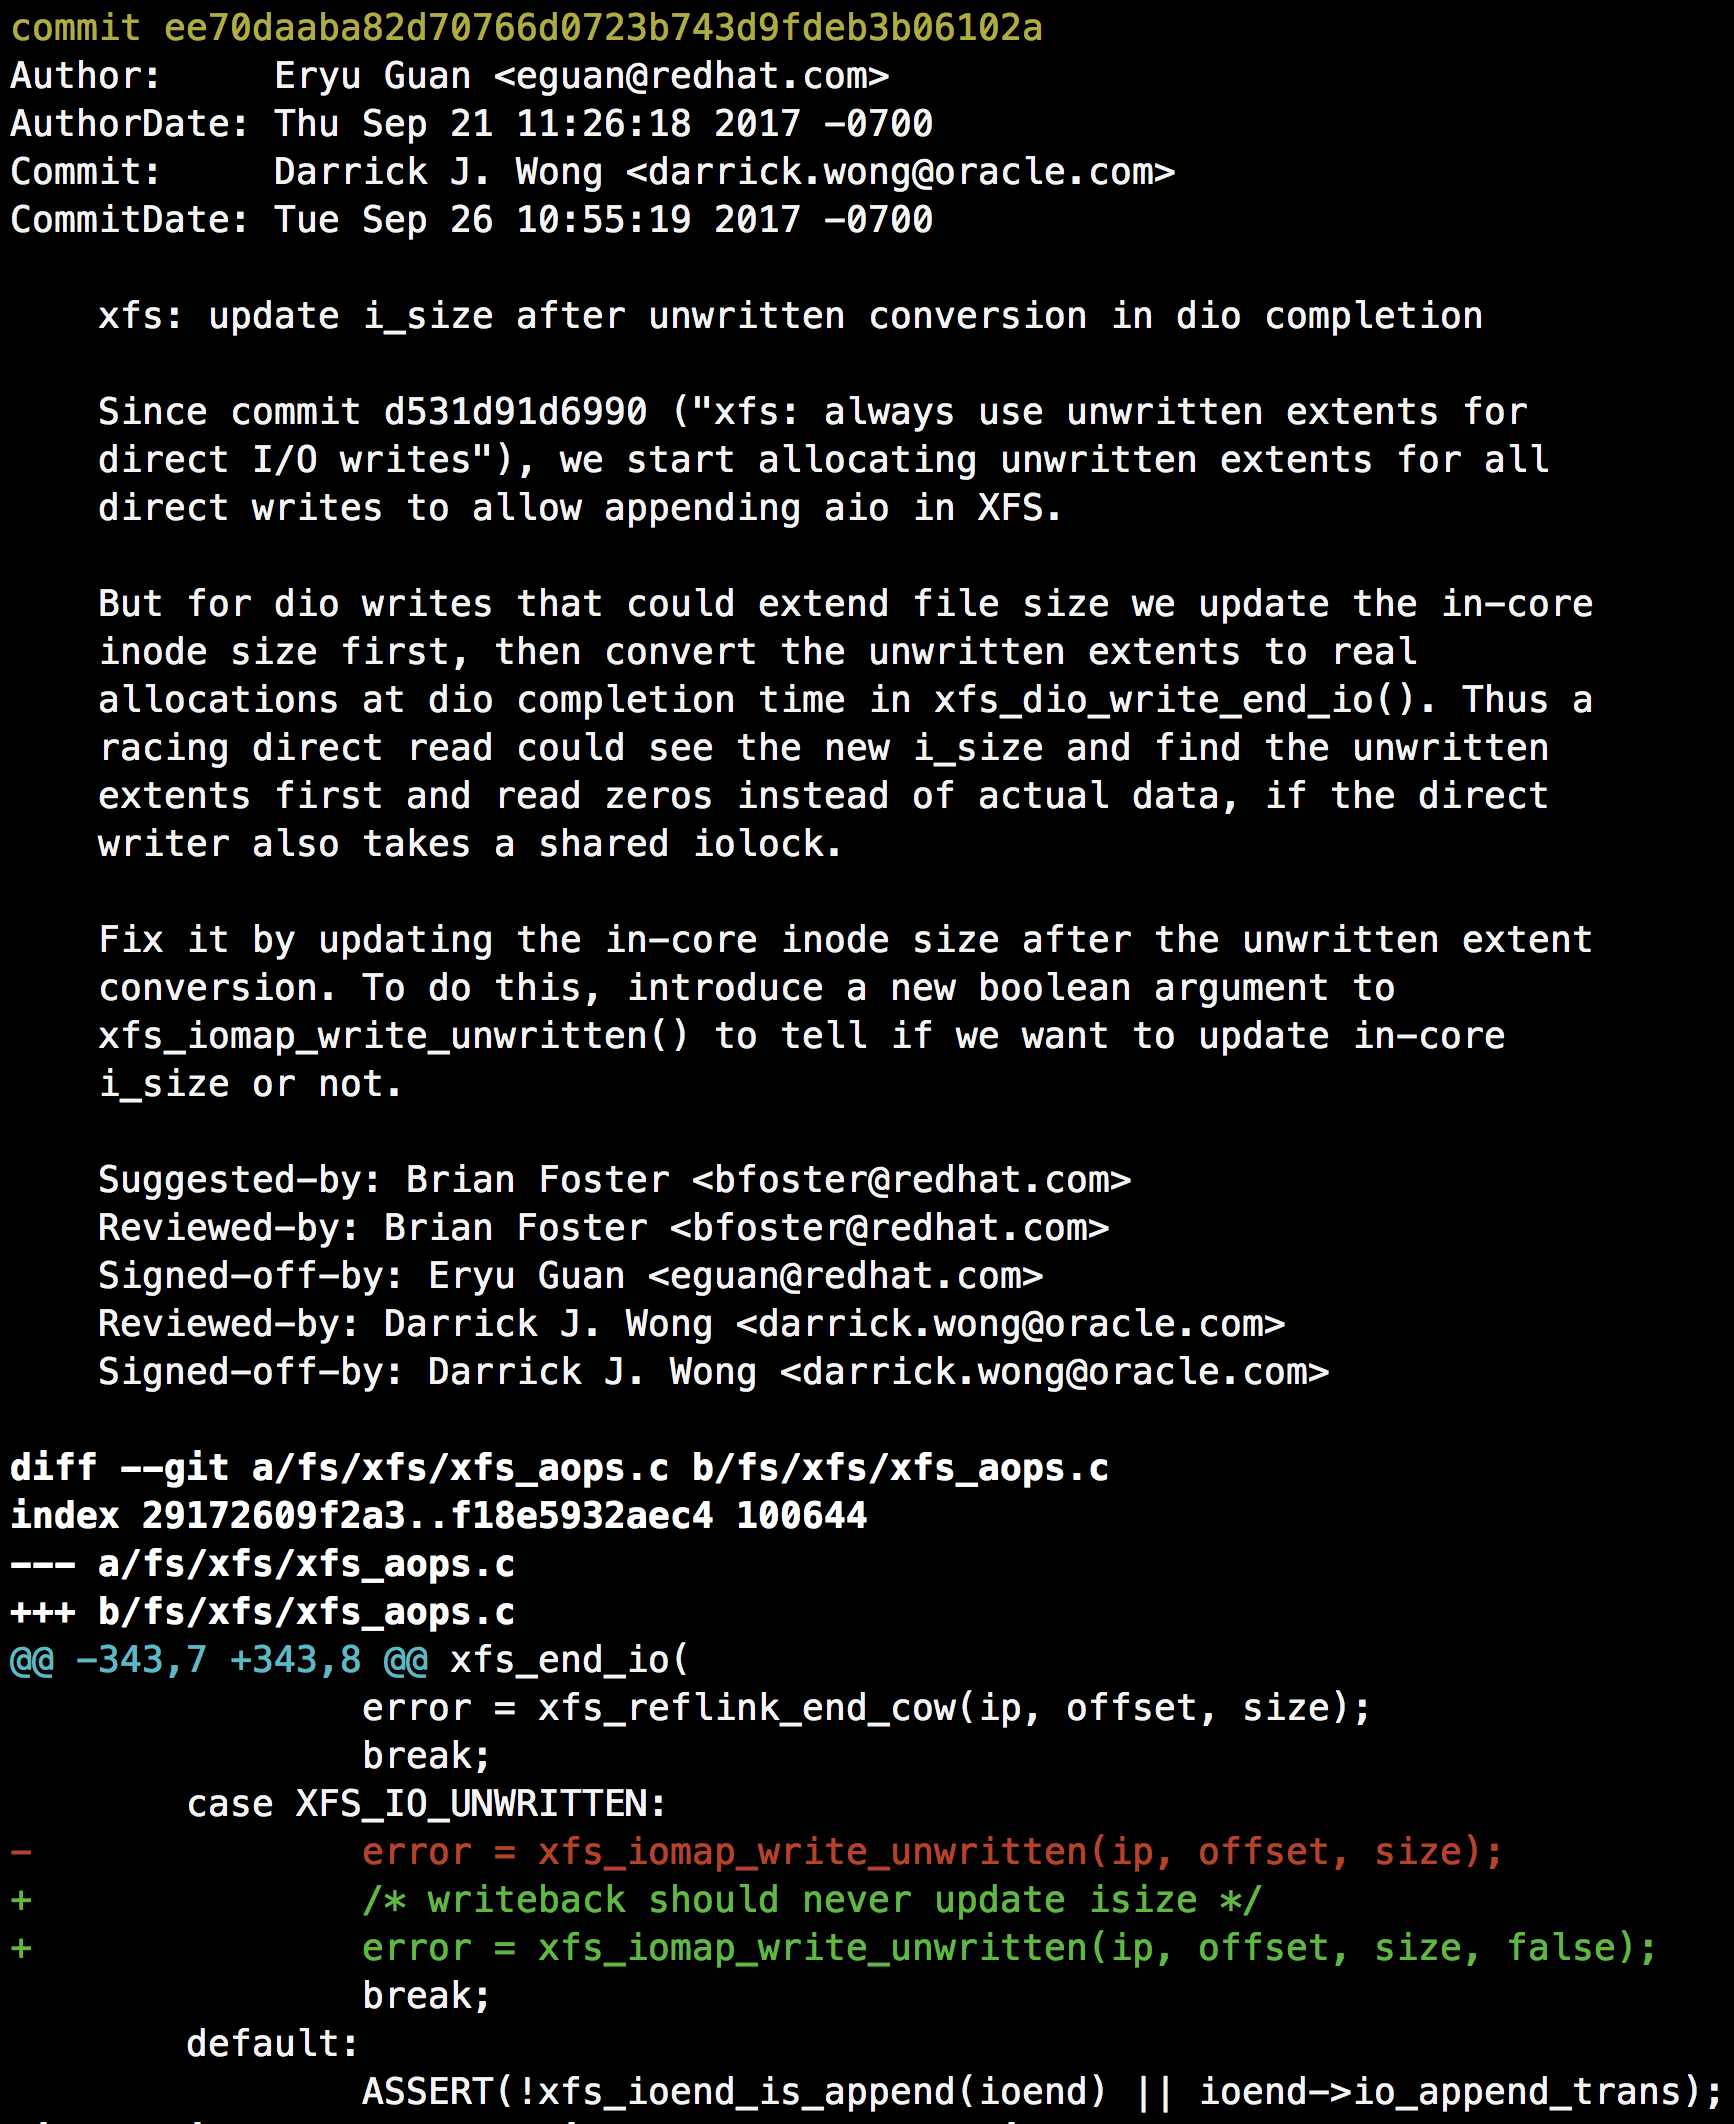
\includegraphics[width=4.5in]{commit_anatomy}
\caption{The anatomy of a commit}
\label{fig:commit_anatomy}
\end{figure}

\begin{itemize}
	\item \textbf{Commit ID:} The commit's unique identifier.
	\item \textbf{Commit Author:} Name and email address of the developer who \textit{wrote}, or \textit{authored} the code change.
	\item \textbf{Author Date:} Time, date, and timezone at which the changes were submitted.
	\item \textbf{Commit Committer:} Name and email address of the person who committed the code to the repository.
	\item \textbf{Commit Date:} Time, date, and timezone at which the commit was committed tot he repository.
\end{itemize}

In the scope of the Linux Kernel, the Commit Author rarely is the Commit Committer. As explained in \autoref{sec:Introduction}, the author is the person who wrote the code, and then submitted it for review as a patch in an email. The commit committer is the person that received, accepted, and commited the changes to their repository.

The commit message contains the following datapoints:

\begin{itemize}
	\item \textbf{Commit summary:} Often called the commit title, a brief explaination of the purpose of the commit. 
	\item \textbf{Commit Message:} In depth explanation of the purpose of the commit.
	\item \textbf{Credit Attribution Tags:} List of people who were involved in the commit and the nature of their involvement. 
\end{itemize}

There are many different types of credit attribution tags, each describing the way the person contributed to the commit. The most common ones, and the ones we use in this study are: \textit{Signed-off-by}, \textit{Reviewed-by}, and \textit{Acked-by} (acknowledged by). The tags have the following meanings\footnote{\url{https://www.kernel.org/doc/html/v4.12/process/submitting-patches.html}}. \textit{Signed-off-by} indicates the developer assisted in the creation of the patch or that she committed it upstream. \textit{Acked-by} is used by developers who were not involved in the creation of the patch but wanted to record their approval. \textit{Reviewed-by} is used to credit developers who contributed reviews to the submitted patch. 

The commit diff, which sits at the end of the git log output, shows the exact files and lines that were modified by the author of the commit. Git uses the commit diffs to apply the changes to the files in the repository. The diff can be perceived as the set of instructions to transform the source code into the desired state.



\section{Open Source Participation}

Previous work studies developers' motivation to participate in \ac{OSS}. ~\citep{Wu-oss} warn that the loosely organized nature of OSS development could be associated with a high turnover rate and in unexpected departures. Other work ~\citep{Rigby}, \citep{Foucault}, \citep{Izquierdo-Cortazar}, \citep{Mockus:2010}, \citep{Torchiano:2011:MPT:1985374.1985379}, and \citep{Ricca:2011:DCT:2022348.2022383} study the impact of a high turn over on the organization. The authors argue that departing developers leave the project with the knowledge they acquired during their time as a contributor, removing this knowledge from the project. We believe that this implies that OSS projects are at risk of knowledge loss and we believe that accurate expertise modeling could assist in addressing this issue.





